\chapter{Natal}


\section{The Embossed Stamps}

The  first  postage  stamps  of  {{wi:Natal}}  were  issued  on  1st  June,  1857.    Unfortunately, while Natal was  quite  early in the field  amongst  the 
world's  stamp-issuing  countries,  its  first  stamps  have  never  enjoyed  the 
esteem  and  popularity  enjoyed  by  the  stamps  just  mentioned  and  by  most 
other 'classic' issues of the world.  

There  was  no  properly  organised  postal  service  in  Natal  until  the  year 
1850.  In terms  of a  proclamation  dated  February  of that  year,  Post  Offices 
were  established  at  Pietermaritzburg,  D'Urban,  Bushman's  River  (later 
Estcourt)  and  Klip  River  (later  Ladysmith).  Previously,  such  limited  postal 
facilities  as  were  called  for  had  been  provided  by  the  various  missionaries 
(mostly  American),  while  between  Pietermaritzburg  and  Durban  the  proprietors  of  the  Natal  Witness  had  provided  what  they  referred  to  as  a 
'Private Post  established  for  the  satisfaction  of  our subscribers.  and  at  the 
same time to afford facilities for communication to the public'.  

This private 
post  commenced  in  March,  1846,  and  was  soon  being  conducted  on  a 
regular weekly  basis,  the tariff  being  6d.  per sheet.  By the time  the  Government  postal  service  commenced  in  February,  1850,  the  tariff  had  been 
reduced to  3d.  per sheet. With  the  establishment  of  the Government service. 
the  private  post  terminated. 

After the opening of the initial four  Government post  offices,  further post 
offices were opened from time to time.  Pinetown and Richmond were opened 
later in  1850,  Verulam  in  1851,  Howick,  Mooi  River,  Colenso, Weenen  and 
York  in  1852,  Sterkspruit  (later  Caversham)  in  1853,  Grey town  in  1854, 
Umhlali in  1856,  Umzinto  in  1858,  Isipingo  in  1859  and  many  more  in  the 
l860s.  By  1870  the  number  of  post  offices  in  the  Colony  had  passed  40 
and by 1880 the number was up to 73.


\begin{figure}[htbp]
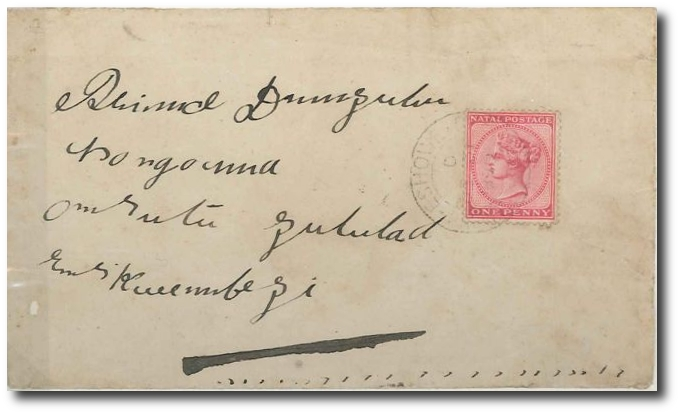
\includegraphics[width=.80\textwidth]{../natal/dinuzulu.jpg}
\caption{
Cover franked 1d, addressed to "Prince Dinuzulu", the Zulu Paramount Chief at Nongoma, cancelled by Eshowe/Province of Zululand c.d.s. of 31 December 1899, backstamped double ring "Nongoma/Natal" c.d.s. of 5 Jan 1900, replacing the fine violet single ring "Nongoma/Zululand" c.d.s. Estimate \euro150. (Part of a larger lot 2012 Feldman).}
\end{figure}

The first stamps of Natal were embossed in relief on plain coloured paper. They were executed at the 
Natal Treasury by May and DDavis, Pietermaritzburg from dies made by William Wyon in London.

More than one reprint was made. They can be distinguished by the brighter colours and clearer embossing than that of the 
original and slightly glazed paper.


\section{1867 Overprints}

These overpints were made to stop the public, using the postage stamps indiscriminately for revenue purposes
and vice-versa. Lorem ipsum dolor sit amet, consectetur adipiscing elit. Sed nibh justo, dictum sed cursus ac, lobortis et lacus. Vestibulum vitae justo enim. Quisque laoreet elementum felis, ut sodales arcu viverra a. Sed molestie odio vulputate sem rutrum a sagittis est rutrum. Morbi dapibus hendrerit magna, sit amet commodo massa posuere sit amet. Duis pharetra quam scelerisque est lobortis fringilla. Maecenas venenatis feugiat lectus, vel facilisis odio pharetra quis. Etiam at nisl eros, sit amet suscipit lorem. Lorem ipsum dolor sit amet, consectetur adipiscing elit. Sed augue nunc, ornare eget congue sit amet, laoreet vel augue. Morbi vel justo quis ipsum adipiscing egestas vitae non est. Vivamus ac quam quam. Nullam pharetra
                                                    interdum mauris, rutrum pulvinar ligula condimentum id. Donec et blandit lorem. 

\begin{marginfigure}
\centering
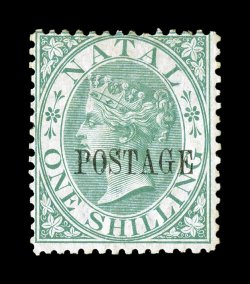
\includegraphics[width=.80\textwidth]{../natal/293.jpg}
\caption{ 
S.G. 31, 1869 1/- Green, with "POSTAGE" overprint, a desirable mint example of a stamp that is missing from even the most advanced collections of the British Empire, sumptuously rich color and a well defined impression, part o.g. with a small paper adherence on the back, fresh and fine; this is the first mint example of this stamp we have ever offered in our auctions and we doubt more than a handful exist; 1997 Holcombe certificate (Scott 37; US9,250.00). (Image) 	\protect\pounds;7,500
SOLD for USD20,000.00}
\end{marginfigure}

Lorem ipsum dolor sit amet, consectetur adipiscing elit. Sed nibh justo, dictum sed cursus ac, lobortis et lacus. Vestibulum vitae justo enim. Quisque laoreet elementum felis, ut sodales arcu viverra a. Sed molestie odio vulputate sem rutrum a sagittis est rutrum. Morbi dapibus hendrerit magna, sit amet commodo massa posuere sit amet. Duis pharetra quam scelerisque est lobortis fringilla. Maecenas venenatis feugiat lectus, vel facilisis odio pharetra quis. Etiam at nisl eros, sit amet suscipit lorem. Lorem ipsum dolor sit amet, consectetur adipiscing elit. Sed augue nunc, ornare eget congue sit amet, laoreet vel augue. Morbi vel justo quis ipsum adipiscing egestas vitae non est. Vivamus ac quam quam. Nullam pharetra
                                                    interdum mauris, rutrum pulvinar ligula condimentum id. Donec et blandit lorem. Lorem ipsum dolor sit amet, consectetur adipiscing elit. Sed nibh justo, dictum sed cursus ac, lobortis et lacus. Vestibulum vitae justo enim. Quisque laoreet elementum felis, ut sodales arcu viverra a. Sed molestie odio vulputate sem rutrum a sagittis est rutrum. Morbi dapibus hendrerit magna, sit amet commodo massa posuere sit amet. Duis pharetra quam scelerisque est lobortis fringilla. Maecenas venenatis feugiat lectus, vel facilisis odio pharetra quis. Etiam at nisl eros, sit amet suscipit lorem. Lorem ipsum dolor sit amet, consectetur adipiscing elit. Sed augue nunc, ornare eget congue sit amet, laoreet vel augue. Morbi vel justo quis ipsum adipiscing egestas vitae non est. Vivamus ac quam quam. Nullam pharetra
                                                    interdum mauris, rutrum pulvinar ligula condimentum id. Donec et blandit lorem. 

\begin{marginfigure}
\centering
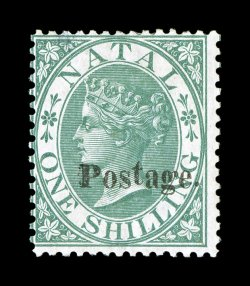
\includegraphics[width=.80\textwidth]{../natal/294.jpg}
\caption{ 
S.G. \#37, 1869 1/- Green, with 12 3/4mm "Postage." overprint, uncharacteristically fresh, with deep intense color and a sharp impression on fresh paper, o.g., h.r., small thin spot at top, otherwise a fine example of this exceedingly rare mint stamp; signed Calves and accompanied by a clear 1997 Holcombe certificate (Scott \#21; \$6,750.00). (Image) \pounds 5,500
SOLD for \$13,000.00 
}
\end{marginfigure}


\end{document}


</div>
<div style="width:32%;float:left">
<img src="http://localhost/egypt/natal/295.jpg" style="width:98%" />
<p style="font-size:smaller"> 
S.G. \#40b, 1869 3p Blue, with 13 3/4mm "Postage." overprint, unused, bright and fresh, fine; a rather elusive stamp, especially unused; 1997 Holcombe certificate (Scott \#23; \$1,900.00). (Image) 	&pound;1,500

SOLD for \$1,500.00	
</p>
</div>
<hr/>
<div style="width:32%;float:left">
<img src="http://localhost/egypt/natal/296.jpg" style="width:98%" />
<p style="font-size:smaller"> 
S.G. \#42, 1869 6p Violet, with 13 3/4mm "Postage." overprint, scarce unused example, bright color, minor thin speck, fine appearance; clear 1968 RPS certificate (Scott \#24; \$1,900.00). (Image) 	&pound; 1,500

SOLD for \$2,600.00	
</p>
</div>

<div style="width:32%;float:left">
<img src="http://localhost/egypt/natal/297.jpg" style="width:98%" />
<p style="font-size:smaller"> 
	S.G. \#48, 1869 6p Violet, with 14 1/2 to 15 1/2mm "Postage." overprint, an exceedingly fresh mint example of a terribly difficult stamp, marvelously rich color on bright white paper, dried o.g., fine; 1997 Holcombe certificate (Scott \#28; \$1,500.00). (Image) 	&pound;1,200

SOLD for \$2,500.00
</p>
</div>
<div style="width:32%;float:left">
<img src="http://localhost/egypt/natal/298.jpg" style="width:98%" />
<p style="font-size:smaller"> 
	S.G. \#49, 1869 1/- Green, with 14 1/2 to 15 1/2mm "Postage." overprint, an incredibly rare mint example, o.g., overall toning, thin spot at left and a few perforation defects, nonetheless a very collectable copy, being the first mint example we have ever offered; 1997 Holcombe certificate (Scott \#29; \$16,750.00). (Image) 	14,000

SOLD for \$5,250.00
</p>
</div>
<hr/>

\#\#\#1870 Curved Postage Overprint

<div style="width:32%;float:left">
<img src="http://localhost/egypt/natal/299.jpg" style="width:98%" />
<p style="font-size:smaller"> 
S.G. \#57, 1870 1/- Green, with curved "Postage" overprint in carmine, strong rich color, reasonably well centered, tiny repair at top right, fine appearance; a very rare stamp that is recorded only in used condition; 1951 RPS certificate (Scott \#41; \$4,500.00). (Image) 	3,500

SOLD for \$10,000.00 	
</p>
</div>
These were overprinted by De La Rue as shown in (a) carmine (b)black or (c) green. There were 96,000 printed and they also
exist with __CANCELLED__ as specimens. They can also be found with the overprint double. Blocks are very
scarce from 20N. On cover they from 2N.

Dangerous forgeries exist of (a) and (b) by painting over the genuine green overprint, which is the cheapest
of the lot.
<hr/>
<div style="width:32%;float:left">
<img src="http://localhost/egypt/natal/300.jpg" style="width:98%" />
<p style="font-size:smaller"> 
&pound;5 Mauve and black, very scarce mint single, attractive colors, 
o.g. that has been toned, fine appearance; 2008 BPA certificate (Scott \#98; \$3,500.00). (Image) 	&pound;2,750

SOLD for \$1,700.00 	
</p>
</div>

<div style="width:32%;float:left">
<img src="http://localhost/egypt/natal/SG141.jpg" style="width:98%" />
<p style="font-size:smaller"> 
10/- deep rose and chocolate, very fine mint. SG 141
	&pound;55 
</p>
</div>
<div style="width:32%;float:left">
<img src="http://localhost/egypt/natal/301.jpg" style="width:98%" />
<p style="font-size:smaller"> 
S.G. \#145b, 1902 &pound;20 Red and green, a seldom seen unused example of this high value rarity, nicely centered, attractive colors, regummed over a light horizontal crease, tiny ink mark by "V" of "Revenue", very fine appearance; signed A. Diena and accompanied by a 2008 BPA certificate (Scott \#100; \$20,000.00). (Image) 	&pound;16,000

SOLD for \$6,000.00	
</p>
</div>
<div style="width:32%;float:left">
<img src="http://localhost/egypt/natal/302.jpg" style="width:98%" />
<p style="font-size:smaller"> 
S.G. \#171, 1908 &pound;1 Purple and black on red, choice quality top sheet-margin single, exceptionally well centered, deep vibrant colors, fresh clean o.g., never hinged (faintly hinged in the selvage only), extremely fine (Scott \#116; for hinged \$350.00). (Image) 	for hinged &pound;275

SOLD for \$700.00
</p>
</div>

<div style="width:80%;float:left">
<img src="http://localhost/egypt/natal/na24.jpg" />
<p style="font-size:smaller"> 
1877-79 QV surcharges. 1/2 d on 1d yellow, 1d on 6d violet and 1d on 6d rose. The set of three fine mint. An attractive group. SG 91-93
</p>
</div>

<hr/>


<div style="width:80%;float:left">
<img src="http://localhost/egypt/natal/108a.jpg" />
<p style="font-size:smaller"> 

Sale 4001 Lot 556

Natal
1888 (Mar.) 1/- orange, variety overprint double, neatly cancelled; reperforated at right and a few other small perf. faults though a presentable example of this rare stamp. R.P.S. Certificate (1955). Sc. 76a; S.G. 108a, &pound;1,500. (WF). Photo
Estimate &pound; 120-150 (sold &pound;80)

Spink Sale 4001 Lot 556. 25 Mar 2004 10:30 London
</p>
</div>

<hr/>


\#\#\#1904 Official

<div style="width:48%;float:left">
<img src="http://localhost/egypt/natal/O2.jpg" style="width:98%"/>
<p style="font-size:smaller"> 
</p>
</div>
<div style="width:48%;float:left">
<img src="http://localhost/egypt/natal/O5.jpg" style="width:98%"/>
<p style="font-size:smaller"> 
</p>
</div>
<div style="width:48%;float:left">
<img src="http://localhost/egypt/natal/O3.jpg" style="width:98%"/>
<p style="font-size:smaller"> 
</p>
</div>



<div style="width:48%;float:left">
<img src="http://localhost/egypt/natal/O6.jpg" style="width:98%"/>
<p style="font-size:smaller"> 
</p>
</div>

                                                                          